\centerline{\bf \huge 7 класс}
\centerline{\bf \huge Решения}

\problem{7.1}
В лесу жили два гнома - Арсений и Вениамин. Арсений врал по понедельникам, вторникам и средам, а Вениамин - по вторникам, четвергам и субботам. В остальные дни они говорили только правду. Однажды при встрече одному из них задали вопрос: «Как тебя зовут?»

--- Арсений, - ответил он.

--- А какой сегодня день недели?

--- Вчера было воскресенье.

Его приятель добавил: «А завтра будет пятница». У приятеля спросили: «Ты говоришь правду?».

--- Я всегда говорю правду по средам, - ответил он.

Кто из них Арсений, кто --- Вениамин и в какой день недели состоялся этот разговор?

\textit{Решение.}
Первый гном не может быть Арсением, а может быть только Вениамином (т.к. если бы это был Арсений, то он говорил бы правду, а утверждение "вчера было воскресенье"\ не может быть правдой из уст Арсения), причём в день разговора он обманывал. Второй гном был Арсений, причём тоже обманывал. Обманывать сразу оба гнома могли только во вторник.

Ответ: первый --- Вениамин, второй --- Арсений, разговор состоялся во вторник.

\problem{7.2}
Малыш подарил Карлсону большую коробку конфет. Карлсон съел все конфеты за три дня. В первый день он съел $\dfrac{1}{5}$ всей коробки и еще 16 конфет. Во второй день $\dfrac{3}{10}$ остатка и еще 20 конфет. В третий день $\dfrac{3}{4}$ остатка и последние 30 конфет. Сколько конфет было в коробке?

%1-2 задачи Краснодар муницип 6 класс 2017 

\textit{Решение.} Пусть $x$ - число конфет, которое было в коробке. В первый день было съедено ( $0,2 x+16$ ) конфет; во второй и третий дни было съедено ( $0,8 x-16$ ) конфет. Во второй день было съедено $(0,3(0,8 x-16)+20)=(0,24 x+15,2)$ конфет; в третий день осталось $(0,56 x-31,2)$ конфет. Так как в третий день было съедено 0,75 остатка и ещё 30 конфет, то остаток будет составлять 120 конфет. Получаем уравнение $0,56 x-31,2=120$, откуда находим $x=270$.

\newpage

\hspace{3mm}

\problem{7.3}
Найдите наименьшее натуральное число, которое при делении на $3,4, \ldots, 9$ даёт остатки $1, 2, \ldots, 7.$ Ответ обоснуйте.

\textit{Решение.} 
Пусть $x$ искомое число. Можно сразу заметить, что $x+2$ делится на $3, 4, \ldots, 9$. Но как до этого дойти самому? Условие нам говорит, что $x\equiv 1 \pmod{3}, x \equiv 2 \pmod{4}, \ldots, x \equiv 7 \pmod{9}$. Заметим, что каждый остаток в каждом сравнении можно заменить на $-2$. Действительно $x \equiv 1 \equiv -2 \pmod{3}, x \equiv 2 \equiv -2 \pmod{4}, \ldots, x \equiv 7 \equiv -2 \pmod{9}$. А это означает, что $x+2$ делится на все число от 3 до 9. А минимальное такое число это НОК чисел от 3 до 9, то есть 2520. А значит $x = 2520 - 2 = 2518.$

\problem{7.4}
В треугольнике $A B C A B=B C$. Точка $E$ лежит на продолжении стороны $A C$ за точку $A$, причём $E A=A C$. Точка $F$ лежит на продолжении стороны $B C$ за точку $C$, причём $F C=C B$. Прямые $F A$ и $B E$ пересекаются в точке $D$. Докажите, что $A D=E D$.

%Тульская область 2024


\begin{center}
    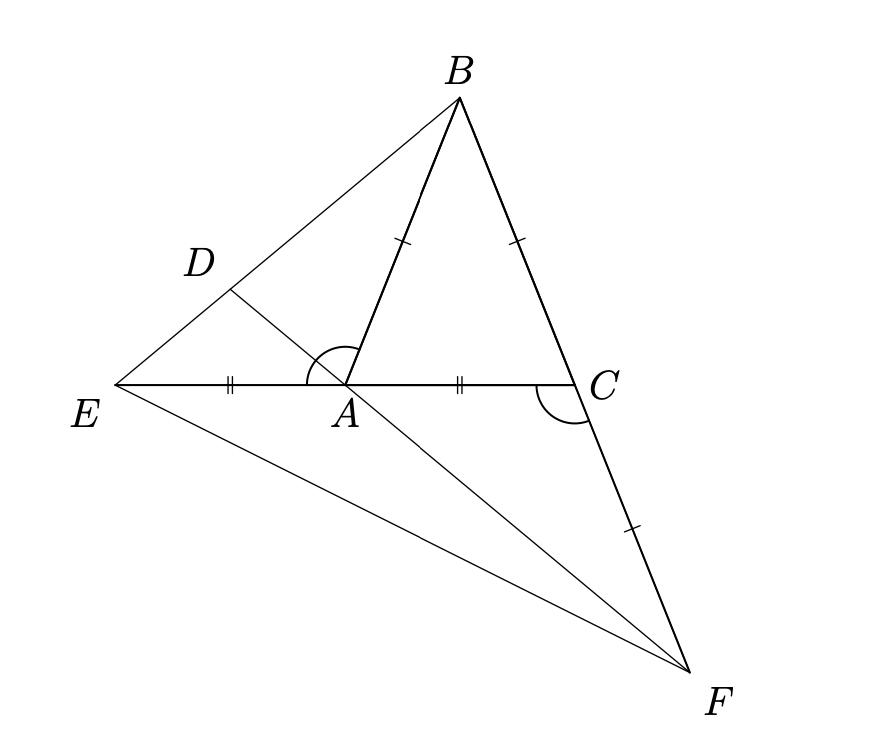
\includegraphics[width=0.5\textwidth]{ЭлМШ 2025-2026/III блок/7/Тренировки/I/Решения/7.4.jpg}
\end{center}

\textit{Решение.}
Углы $B A C$ и $B C A$ равны, а значит смежные с ними углы $B A E$ и $A C F$ тоже равны. Тогда треугольники $E A B$ и $A C F$ равны по двум сторонам и углу между ними. Тогда $\angle A E B=\angle C A F$. Но, так как углы $C A F$ и $D A E$ вертикальные, то они равны, а значит $\angle A E D=\angle D A E$, откуда треугольник $A D E$ - равнобедренный, и $E D=A D$.